\documentclass[aps,prl,preprint]{revtex4}
%\documentclass[aps,prd,twocolumn,twoside,floatfix]{revtex4}

\usepackage{pioneer}
	\def\theAuthor{Tony Lu}
	\def\theYear{2016}
\usepackage{graphicx}
\usepackage{bibentry}

\begin{document}
\pagestyle{pioneer}
\date{April 2016}
\preprint{}
\title{Background of LIGO}
\author{Tony Lu}


\begin{abstract}
Because of the first detection of gravitational waves, Albert Einstein's General Theory of Relativity and the Laser Interferomter Gravitational-wave Observatory (LIGO) suddenly became one of the most popular topics. This document is to present background information about LIGO and gravitational waves.

\end{abstract}

\maketitle

\section{Introduction \label{intro}}
More than one hundred years ago Albert Einstein's General Theory of Relativity \cite{relativity1, relativity2} states, we live in a four dimensional world--spacetime (three dimensions for space and one for time). Masses cause distortions in spacetime, which accounts for the phenomenom of gravity. And the theory predicts that changing mass distribution will generally produce ripples in spacetime, which is Einstein's another prediction--gravitational waves. For decades, scientists have been struggling to detect gravitational waves from the outer space. They upgraded their detectors over and over again, just in order to catch the whisper from distant celestial bodies. Fortunately, on September 14, 2015, the LIGO detectors successfully recorded the signals from two colliding black holes, which was the first direct detection of gravitational waves ever, a remarkable one.  \cite{GW}

This actual detection is evidently significant. Einstein was proven right again, a new field of astronomy has been opened, new possibilities of universe study are found, increasing research on gravitational waves and astronomy will be spurred, and so on. The issue will be addressed in more detail later in the paper.

The goal of this document is to provide background information about LIGO and gravitational waves. The paper starts with some brief information about LIGO, consisting of an introduction to gravitational waves (without much math and calculation),d technical details of LIGO detectors, its history (stages went through), its impact on modern science, and some of the related projects.
%=============================================================


\section{A Brief Introduction to LIGO \label{BI2LIGO}}
The Laser Interferometer Gravitational-wave Observatory (LIGO) is a large-scale cutting-edge physics experiment which aimed to detect and successfully detected gravitational waves. The LIGO detectors at the LIGO Livingston Observatory (LLO), in Livingston Parish, louisiana, and the LIGO Hanford Observatory (LHO), in Hanford, Washington, are funded by the National Science Foundation (NSF), and are operated by Caltech and MIT. There are plenty of similar projects all over the world, such as VIRGO \cite{Virgo} and eLISA \cite{eLISA}.

From the 1990s up to the present, LIGO went through several stages, with increasing sensitivity and functions, and it had been bearing doubts. In September, 2015, just a week after the advanced LIGO was set into \emph{observing} mode, a signal which was later confirmed to be generated by two colliding black holes was detected. \cite{GW} And the LIGO scientists made their official report in February, 2016. \cite{O1}
%================================================================


\section{Introduction to Gravitational Waves \label{intro2GW}}
This section addresses gravitational waves--the theory that predicts it, its properties, the possible sources, and about its detection.

\subsection{The General Theory of Relativity}
In order to describe gravity, Einstein developed, on the basis of his Specific Theory of Relativity \cite{spe.relativity}, a theory system named the General Theory of Relativity (General Relativity), which was proposed in 1915. \cite{relativity1} Despite the fact that the theory is still in contradiction with quantum theory, and that it was so complex that it took 40 or more years for most physicist to reach an agreement on it, it has successfully accounted for and predicted numerous phenomena, such as time dilation in gravitational fields, red shift of light, and gravitational waves.

The core idea of General Relativity is that gravitation i s described as a property of the geometry of spacetime which includes three dimensions for space and one for time. To be more precise, the principles state that matter curves spacetime, and objects, which maybe in a \emph{free-fall}, travel in straight paths. As a result, although objects are actually traveling in straight paths in the presence of gravity in spacetime, they are observed to be traveling in curved trajectories. The more massive an object is, the more curvature it will create in spacetime, which results in more gravitational force. And the curvature is often expressed with Riemann curvature tensor. \cite{Tensor,wikitensor}\newline
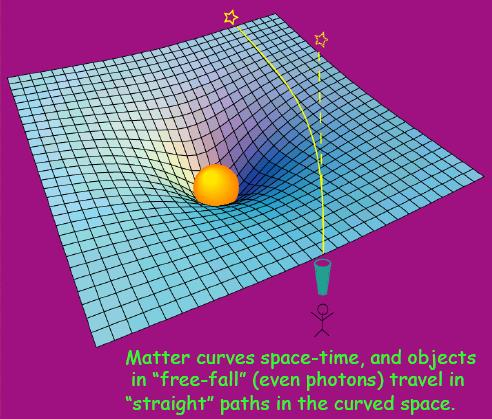
\includegraphics{curvature}

\subsection{Properties of Gravitational Waves}
Gravitational waves are \emph{ripples} in the \emph{fabric} of spacetime, caused by some strong and catastrophic happenings in the universe. More technically, they are changing gravitational fields varying with time.

According to Einstein's calculations, gravitational waves are generated by objects acclerating with asymmetric motion. To be more precise, gravitational waves require changing quadrupole mass distribution. \cite{SBackground} The amount of gravitational waves given off is of positive correlation to its mass and its speed of motion. Changes in spacetime produced by a moving mass are not felt in the distance at once, but they propogate at the speed of light.

Gravitational waves are tranverse waves, the same as electromagnetic waves, but they are waves of changes in tensors (quadrupole distortions of spacetime) which result in expansions and contractions in lengths in certain directions. Unlike the horizontal and vertical polarizations of electromagnetic waves, the two polarizations of gravitational waves are long the + and $\times$ direction. However, gravitational waves do share lots of similarities with electromagnetic waves. They have frequencies and wavelengths, whose relationship is given by: $\lambda f=c$, where $\lambda$ is the wavelength, $f$ is the frequence, and c is the speed of light. They are able to carry energy, momentum, and angular momentum away the source. \cite{SBackground} The strain amplitude can be derived from Einsteins quadrupole formula \cite{relativity2}, and it can also be measured by ratio of the change in length to the original length $h=\frac{\Delta L}{L}$.

\subsection{Sources of Gravitational Waves}
There are various sources that can emit gravitational waves, but they fall mainly into 4 catagories: stochastic backgroud, bursts from gravitational collapse, pulsars, and binary systems.

Stochasic background results from superposition of countless discrete systems and from some fundemental process, like the Big Bang. The radiation from the Big Bang, if really detected, can provide us with insights of the very nature of physics and the secret of the universe. \cite{SBackground}

Bursts from gravitational collaps can be produced by the process during which a highly-evolved celestial body undergoes a gravitational collaps, becoming a neutron star or a black hole. If the collapse is nonspherical, binding energy or angular momentum will be carried away by gravitational waves. \cite{SBackground}

Stars with imperfectly spherical shape also emit gravitational waves while rotating. Although the all the mass is belongs to a single unity, the uneven distribution of mass during rotation leads to varying quadrupole tensor (namely, gravitational waves).

Binary systems refer to those that consist of two bodies rotating aroung each other. Whether or not the two stars collide, gravitaional waves will be generated. The detection made on September 14, 2015 is the collision of two black holes. \cite{SBackground}

More details are given by \cite{SBackground} in section 3.

\subsection{Possible Way of Detection}
Due to the properties of gravitational waves, they cannot be measured quatitatively in a conventional way, even though they might be significant enough to be observed with bare eyes. When passing by, gravitational waves distort the space. As a result, a meter stick would also be distorted, therefore impossible to measure the change in length.

One plausible solution would be a piezoelectric detector, which when deformed, generates voltage between the two disks. \newline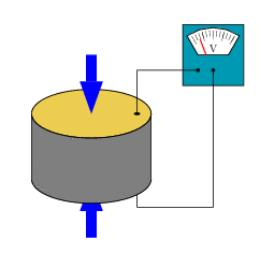
\includegraphics{Piezoelectric}\newline But it hadn't been sensitive enough to respond to the infinitesimally small change in length, so it finally failed. However, there's a value in the universe which always remains constant against all odds--the speed of light. Armed with this property, lights can ignore the deformation of spacetime, and show the changes in arm length with different time or distance traveled. Scientists have made the detector in a way such that light have to travel over 1000 km \cite{Interferometer} to reach the detector, which greatly strengthened the sensitivity and increased the odds of detection.
%=============================================


\section{Technical Details of LIGO \label{TechLIGO}}
This section presents the LIGO in more details, including its core technology, its current obervatories, and the most important issue--sensitivity.

\subsection{Michelson Interferometer}
The Michelson Interferometer was invented by Albert Abraham Michelson, first used in the famous Michelson-Morley experiment. It's function is for optical interferometry. With a beamsplitter, a light source is split into the two arms, and each of the new beam are reflected back and are combined again. The result of such combination could be constructive or destructive interference, depending on the changes in length of the arms.

The interferometer in LIGO consists of two vacuum arms \cite{MITLIGO} of equal length (4km long) \cite{MITLIGO}, which form an L shape. There is a laser light source and a photodetector at about the corner of the L, and a beamsplitter at the corner. At each end and in the middle of the arms freely hanged four mirrors which reflects the laser beam \cite{Interferometer}, and the two beams are combined into one at the beamsplitter. Those mirrors in the middle are used to increase the distance light beams travel, and as a result, the actual effective length is increased from 4km to 1120 km \cite{Interferometer}, greatly enhancing LIGO's sensitivity. \newline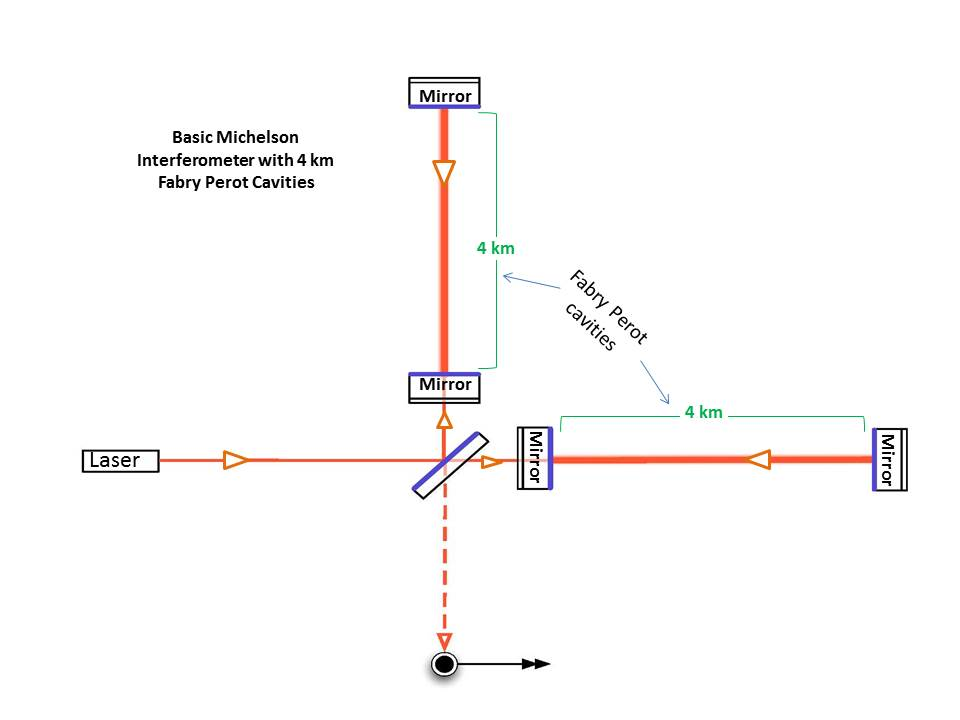
\includegraphics[height = 8cm, width=8cm]{LIGOInterferometer}\newline If the arm length changed, the two light beams which were originally in phase would be out of phase, creating destructive interference which allows the photodetector to sense the infinitesimal change in length of the arms. \newline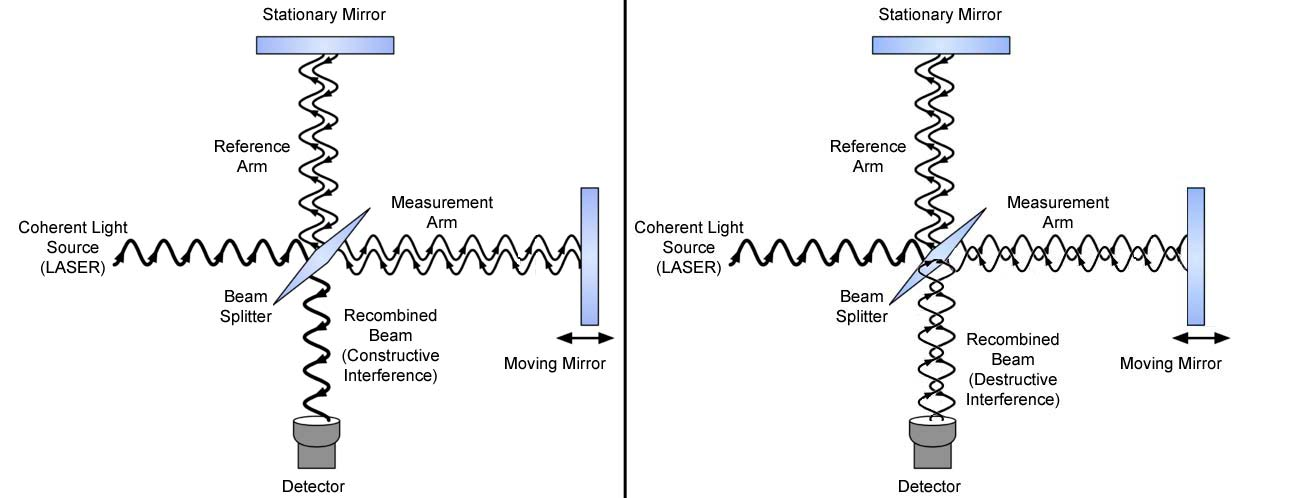
\includegraphics[height=5cm, width= 10cm]{Interferometer}

\subsection{The LIGO Observatories}
The two LIGOs in the US are located in Livinston Parish (LLO), Louisiana and Hanford (LHO), Washington. Both are L-shaped and of the same size--their arms are all 4km long. The two Ls are in different directions, and they are separated by 3030.3km (by Google Earth) on land, which means the planes these observatories are on have an dihedral angle of 27.3 degrees. Therefore, it's guaranteed that gravitational waves from any directions can be detected, given enough sensitivity.

\subsection{Detector Sensitivity--Problems and Solutions}
Like any real physics experiment, the LIGO detectors face various disturbance from the environment. Considering the small amplituded of gravitational waves, we see that sensitivity and the ability of anti-interference become deciding. At the very beginning of the construction, the interference of the noises are so high that it was even impossible for the detectors to collect data clean enough to analyze. But the quality of data collected has been significantly improved over the several stages of LIGO. Among all these sensitivity-limiting factors are majorly: seismic noise (at relatively low frequencies), thermal noise (at mid frequencies), shot noise (at high frequencies), and the problems with the lasers and electronics. \newline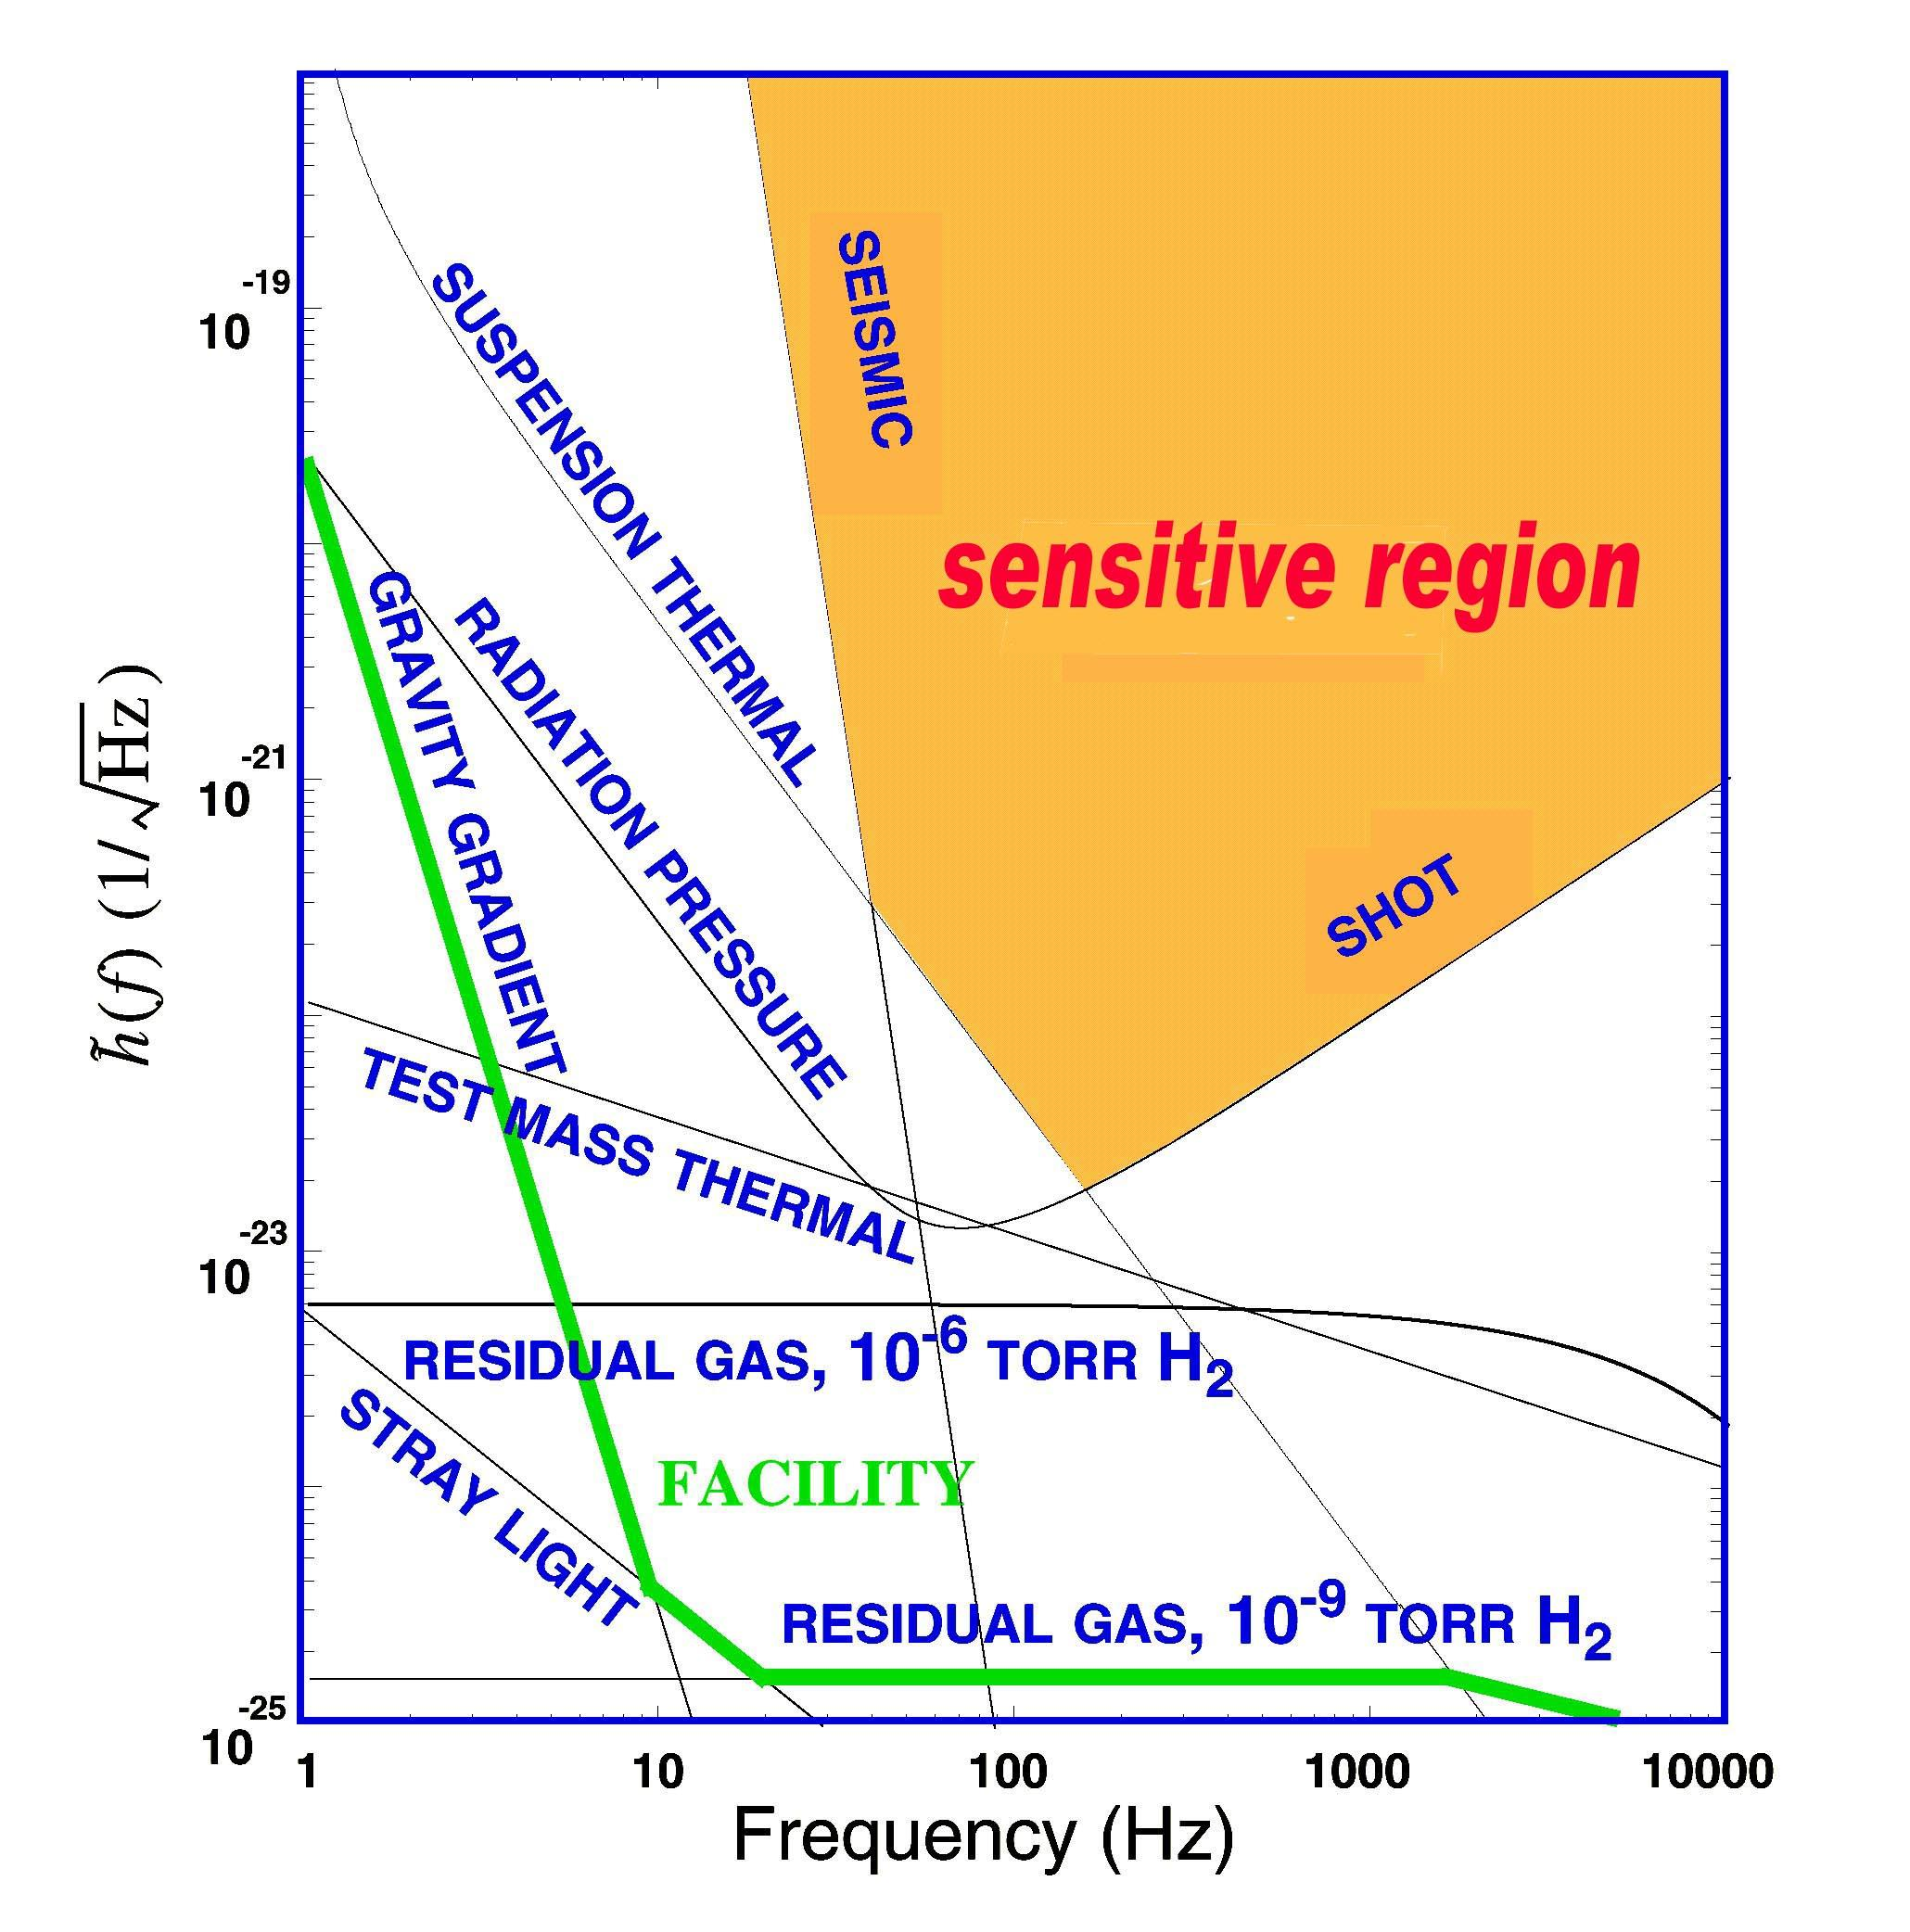
\includegraphics[height=8cm, width=7cm]{SensitiveGraph}

Seismic noises are the disturbance generated by the movement of the earth. They are usually of relatively low frequencies but huge amplitudes. In general, the method to reduce such noise is by manipulating the data through auxiliary subsystems and channels. More details about seismic noise alleviation is given by \cite{seismic}.

Thermal fluctuations (atomic vibrations) are deemed to be the most significant noise of the early LIGO detectors. They are generated by the thermal agitation in the charge carriers such as electrons. These noises can be calculated using the method stated detailedly in \cite{thermal}.

Shot noise is associated with the particle nature of light. The situation can be evidently improved by mutiplying the number of passes in the arms of interferometer. More details are given in section 4.4.1 and section 5 in \cite{Noise}.

Some more specific details are given by \cite{Noise}, especially in the fourth section.

\subsection{Einstein@Home}
Einstein@Home is an astronomy project that relates to LIGO. It is aimed to find out continuous sources of gravitational waves and determine the systems' locations in the sky, using the data collected in each of LIGO's runs. To learn more about Einstein@Home, please visit its homepage. \cite{Einstein@Home}
%===========================================


\section{A Brief History of LIGO \label{history}}
Tracing back to the 1960s, there was an attempt by Joseph Weber detect gravitational waves. He claimed to have detected gravitational waves, but the results then were largely doubted. At the meantime, pioneered by Rainer Weiss at MIT and Ron Drever at Glasgow, prototype interferometers which later became the one thing that enables human beings to hear the call of the universe were being developed.

An experimental gravitational group was promoted in the late 1970s at Caltech by Drever and Stan Whitcomb. And in the 1980s, when LIGO were still prototypes, the US National Science Foundation started funding the construction of them.

During the next few decades, LIGO went through several stages: first official construction (1994-95) \cite{timeline}, Enhanced LIGO and Advanced LIGO approved (2008) \cite{BHLIGO}, Advanced LIGO (2014) \cite{timeline}, and AdvLIGO's sensitivity passing the initial one(2014-15) \cite{timeline}. Both eLIGO and advLIGO had significantly increasing sensitivies over the previous ones, and eventually advLIGO accomplished a sensivity of tenfolds! \cite{BHLIGO}

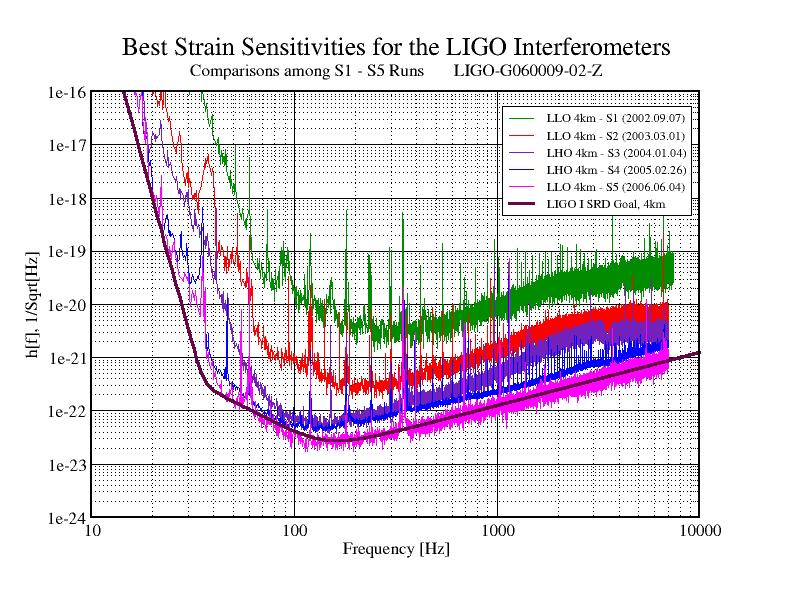
\includegraphics[height = 8cm, width = 10cm]{LIGOsensitivity}

On September 14, 2015, just a few days after being switched into "observe" mode, LIGO detected a quite strong signal which is believed to be gravitational waves from two colliding black holes, and the official report was released on Feburary 11, 2016, referred to as \emph{Observation 1}. \cite{O1}

More details are given by \cite{BHLIGO}.
%===============================================


\section{The Impact of Detection \label{impact}}
As the very first detection of gravitational waves, the event certainly marked a milestone not only in astronomy but also in human history. Such an unprecedented discovery does have a profound impact on science.

To begin with, Einstein's General Theory of Relativity is again proven right. Spacetime is observed in a dynamic state for the first time. But the study is far from over. There still are mysteries about gravitons, which are believed to be the particle that carries the gravitational force, and about black holes themselves. \cite{Impact}

More importantly, the detection of gravitational waves opened a brand new branch of astronomy. Now scientists have more methods to observe the universe. For example, it's almost impossible to study the behavior of black holes with telescopes, because they hardly emit any electromagnetic waves. But they sometimes do transmit gravitational waves. \cite{SBackground} Besides, gravitational waves travel through objects unaffected, \cite{GWTravel} so the information carried is highly authentic.

Furthermore, LIGO is seen also as a legacy for the future. With those new ways of viewing the universe, it can be expected that more and more rules of physics can be found, and eventually we might obtain a really fundamental understanding of physics and the universe. \cite{Impact}


%================================================

\section{Other Cognate Projects \label{other proj.}}
Aside from the two LIGOs in the US, quite a number of observatories for gravitational-wave detection have been established all over the world, or are now under construction. Part of those is listed below, with their websites attached:
	\begin{enumerate}
	\item VIRGO--a giant laser interferometer designed to detect gravitational waves, in Cascina \cite{Virgo}
	\item eLISA--Laser Interferometer Space Antenna  \cite{eLISA}
	\item KAGRA--a laser interferometer observatory in Japan \cite{KAGRA}
	\item GEO600--a ground-based interferometric gravitational wave detector located near Hannover, Germany \cite{GEO600}
	\end{enumerate}

All of these observatories will contribute to the expanding research on gravitational waves.
%====================================================

\section{Summary}
The Laser Interferometer Gravitational-wave Observatory is a ground-based detector aiming to detect and successfully detected gravitational waves. Its prototype is the Michelson Interferometer. With changes in configuration, LIGO evolved over time and eventually reached the required sensitivity. A real detection was made in September 14, 2015. It has had, and surely will continue to have profound impact on science, as well as the whole society. LIGO, along with many other "brothers", will keep on advancing in the new branch of the astronomy.


\bibliography{Paper1Background}
\end{document}